\section{Analisi Etnografica}
Un applicazione può rivolgersi a diverse tipologie di utenti.
L'etereogenità di persone che al giorno d'oggi sono tecnologicamente in
grado di utilizzare smartphone e tablet è elevata, anche se va
considerato che esistono molteplici target d'utilizzo che si
differenziano per varie caratteristiche (e.g. fascie d'età, livello
d'istruzione, genere, stato civile, etc.).

Nello specifico, un applicazione di cucina abbraccia sicuramente più di
una singola tipologia d'utente. 
Ad esempio ci si potrebbe aspettare interesse verso tale applicazione
da parte di utenti 
con una predisposizione tecnologia, molto tempo
libero e medio interesse alla cucina, i quali sarebbero tentati di
affacciarsi al mondo culinario, ma anche di utenti poco informatizzati ma la
quale gran passione per la cucina li porta a compiere lo sforzo di
apprendere il funzionamento di software ideato per la
loro passione. \\

Identificare i diversi target d'utilizzo è fondamentale per comprendere
al meglio come strutturare un applicativo software in quanto tipologie
di utenti divere si relazionano con esigenze diverse.

A tal proposito è stata condotta un'analisi etnografica che di seguito vedremo nel dettaglio. 

\subsection{Segmentazione del Target}
Al fine di individuare una categorizzazione di utenti in sottogruppi
omogenei per qualche caratteristica si fa fronte a due tipi di
segmentazione.

\subsubsection{Segmentazione Demografica}
Per comprendere meglio come segmentare l'utenza abbiamo considerato
attuali studi in letteratura che identificano caratteristiche
demografiche utili al nostro caso.
Nello specifico:
\begin{itemize}
\item Utilizzo demografico degli smartphone statutitesi nel 2014.
\begin{figure} [H]
	\centering
	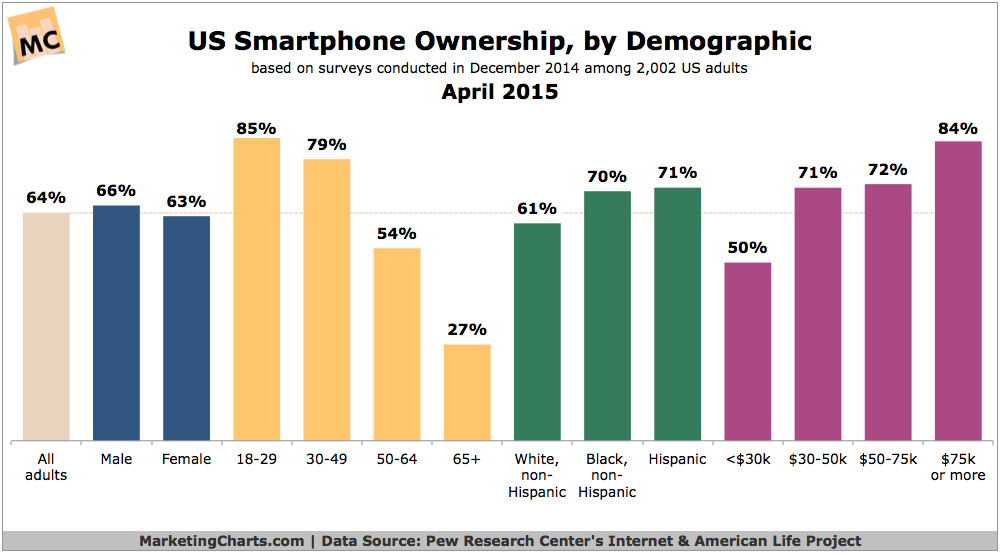
\includegraphics[scale=0.3]{img/demographic-smartphone.png}
\end{figure}
Dal grafico si envince che la ormai l'utilizzo degli smartphone è
estremamente diffuso in quasi tutte le categorie demografiche.
I meno soggetti all'utilizzo di smartphone sono gli individui con un età
che supera i 65 anni.

\begin{minipage}{0.45\textwidth}
\item
Crescita di interesse per la cucina.\\
Recenti articoli parlano di come
ci sia sempre più interesse verso l'arte culinaria. 
Si può riscontrare anche dal gran numero di programmi televisi in voga
negli anni. Inoltre si possono incontrare sempre più blog e canali
youtube nel web di appassionati di cucina che condividono le loro
ricette ed esperimenti.
La condivisione è una proprietà intrinseca della passione culinaria: le
nostre nonne hanno sempre conservato il libro delle ricette personali da
ampliare con le collezioni di ricette passate da amiche e parenti.
Indubbiamente questo fenomeno è esploso con il web e c'è sicuramente
spazio di mercato per applicazioni che permettono di coltivare la
passione culinaria.
\end{minipage}
\begin{minipage}{0.45\textwidth}
\begin{figure} [H]
	\centering
	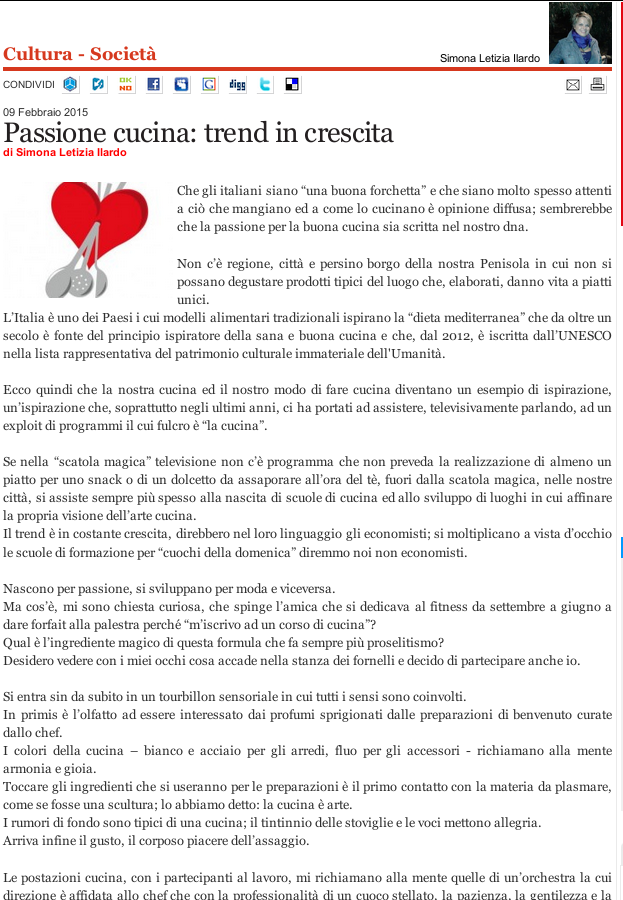
\includegraphics[scale=0.3]{img/articolo-cucina.png}
\end{figure}
\end{minipage}

La figura \ref{fig:demographic-coockapp} riassume uno studio statistico
condotto in Gran Bretagna nel 2013 che mostra la diffusione
dell'utilizzo di applicazioni per cucinare caratterizzata per età e
sesso. In particolare si può notare che c'è un maggiore utilizzo da
parte delle donne e per le persone sotto i 50 anni anche se la
distribuzione di utilizzo è piuttosto omogenea.

\begin{figure}[H]
	\centering
	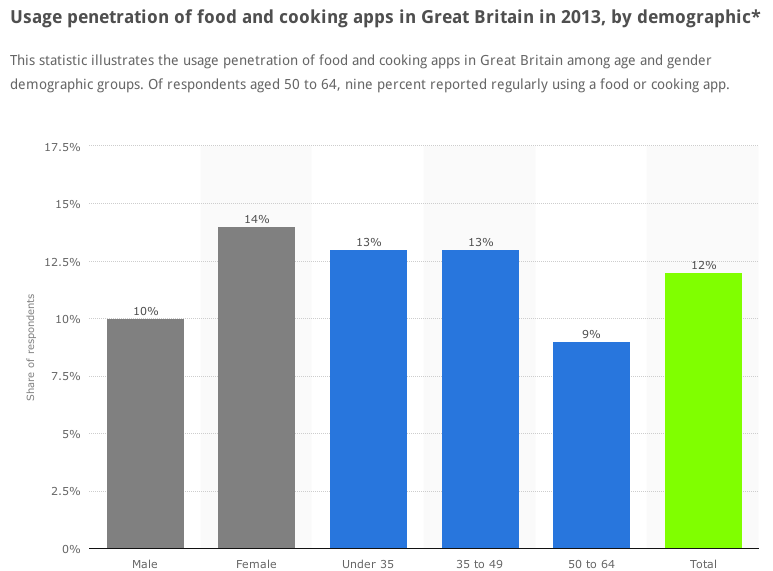
\includegraphics[scale=0.3]{img/demographic-cookapp.png}
	\caption{Diffusione demografica delle applicazioni culinarie in Gran Bretagna nel
2013}	
	\label{fig:demographic-cookapp}
\end{figure}

Inoltre come si evince dalla figura \ref{fig:cooking-country}, ci sono
nazioni in cui la passione per la cucina è importante a differenza di
altre. In particolare l'Italia risulta essere prima in classifica per
passione culinaria.
Questo suggerisce la possibilità di progettare un'applicazione culinaria
specifica per la cucina italiana, la quale da se offre sicuramente un mercato
interessante, senza però escludere la possibilità di
coltivare la passione per la cucina internazionale. 
Un approccio meno specifico e più internazionale rischierebbe di
confondere l'utente medio italiano più legato ai ricettari classici
della cucina italiana. 

\begin{figure}[H]
	\centering
	
\includegraphics[scale=0.7]{img/cooking-country.jpg}
	\caption{Nazioni a confronto riguardo la passione culinaria}	
	\label{fig:cooking-country}
\end{figure}

\end{itemize}

Da quanto visto emerge un target ideale d'utilizzo che si differenzia per ogni
caratteristica demografica:
\begin{itemize}
\item \textbf{Età}. La fascia d'età di maggior interesse è dai 13-65
anni. Non esclude gli over 65 se con una particolare predisposizione
alla tecnologia.
\item \textbf{Sesso}. Qualsiasi: anche se le donne hanno mostrato avere più
interesse nella cucina rispetto agli uomini, il divario è minimo e rende
così l'applicazione indipendente dal sesso.
\item \textbf{Reddito}. Qualsiasi:
in genere le ricette presenti nelle applicazioni culinarie hanno diverse
fasce di prezzo rendendo quest'ultime indipendenti dal reddito dell'utente.
\item \textbf{Nazionalità}. Prevalentemente italiana. Non esclude gli
appassionati per la cucina italiana di diversa nazionalità.
\item \textbf{Istruzione}. È sufficiente possedere una cultura di base sulla terminologia
culinaria e sulla conoscenza delle materie prime più comuni. Si prevede
ovviamente che l'utente sia alfabetizzato e che comprenda le lingue
dell'applicazione. 

\end{itemize}

\subsubsection{Segmentazione Psicografica}
Al fine di identificare al meglio le tipologie di
utenti interessati all'applicazione proposta, abbiamo segmentato
ulteriormente l'utenza, in questo caso individuando le loro caratteristiche
psichiche.

\begin{itemize}
\item \textbf{Intraprendente}
\item \textbf{Insicuro}
\item \textbf{Ansioso}
\item \textbf{Curioso}
\item \textbf{Salutista}
\end{itemize}


\subsection{User Research}

\begin{itemize}
\item Confronto di vendite tra tablet, laptop e desktop nel corso degli utlimi
anni.

\begin{figure} [H]
	\centering
	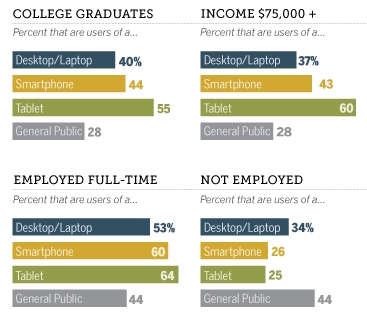
\includegraphics[scale=0.3]{img/Pew-Dems-of-Tablet-Users.jpg}
\end{figure}
Si può notare che la stima di vendite per i tablet è in crescita per i
prossimi anni rispetto a desktop e laptop che sembra rimanere stabile.
Questo suggerisce che per applicazioni general purpose può essere
interessante orietantarsi verso implementazioni tablet.

\item Confronto smartphone tablet
\begin{figure}[H]
	\centering
	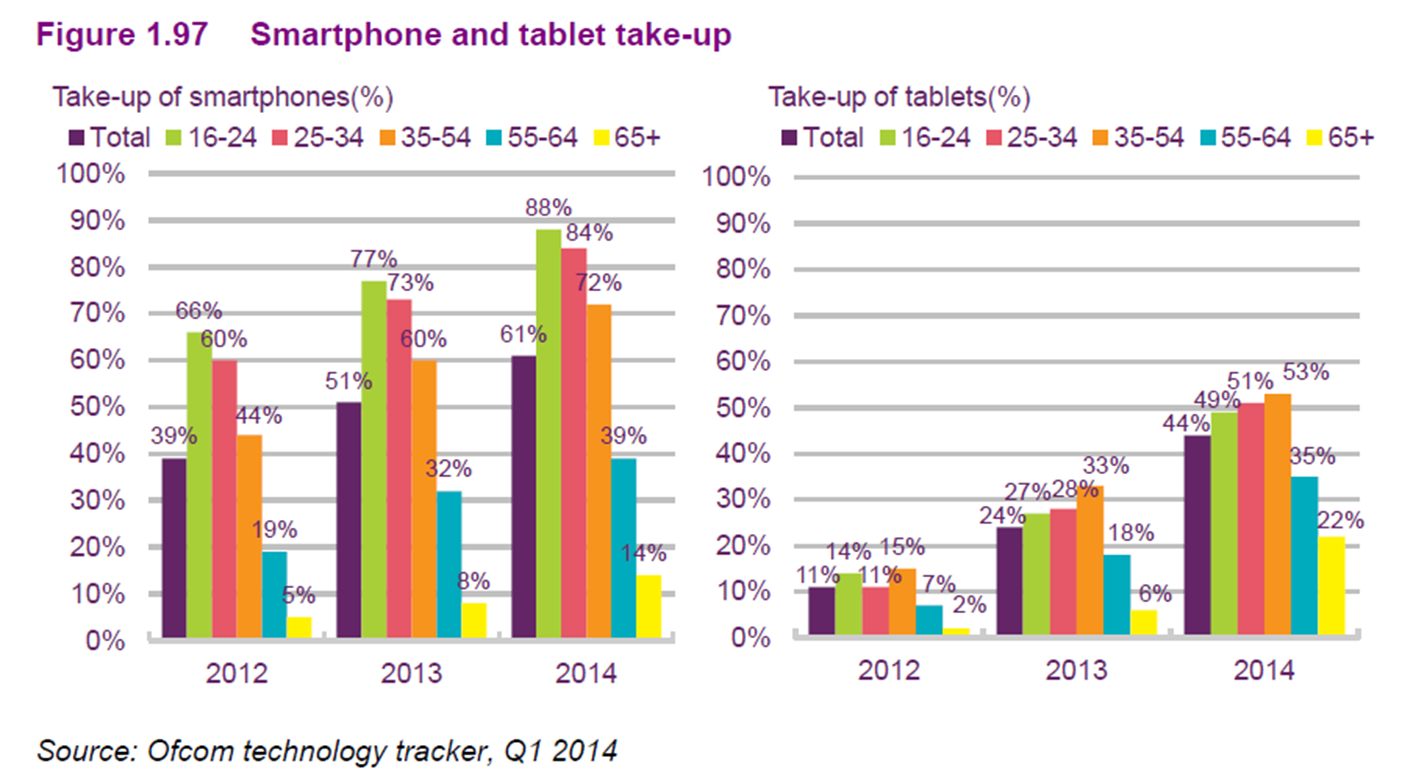
\includegraphics[scale=0.5]{img/Smartphone_Tablet_Age.png}
\end{figure}
\end{itemize}

%TODO stessa cosa per smartwatch
